\icode{O-MD-CA-L2-261115-005}
如图所示，质量为\(m_1\) 的木块 \(A\) 和质量为\(m_2\) 的木块\(B\)通过不可伸长的轻绳连接，当竖直恒力 \(F\)分别作用于上端\(B\)，使\(A\)、\(B\)一起向上加速运动。求\(A\)、\(B\) 间轻绳上的作用力大小。

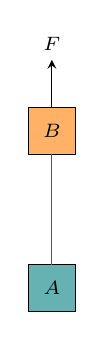
\begin{tikzpicture}[>=stealth,font=\scriptsize]
	\draw[fill=teal!60] (-.3,0) rectangle(.3,.6)node[midway]{\(A\)};
	\draw[fill=orange!60] (-.3,2) rectangle(.3,2.6)node[midway]{\(B\)};
	\draw[->] (0,2.6)--(0,3.2)node[above]{\(F\)};
	\draw[magenta] (0,.6)--(0,2);
\end{tikzpicture}
\begin{answer}
    
\end{answer}